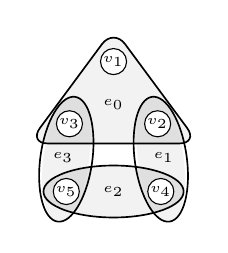
\begin{tikzpicture}[
    scale=1.0,
    every node/.style={transform shape},
    vertex/.style={
        circle, draw, fill=white, font=\tiny,
        minimum size=0.33cm, inner sep=0.4pt
    },
    hfill/.style={
        draw=none, fill=gray!22, fill opacity=0.45
    },
    hint/.style={
        draw=none, fill=gray!50, fill opacity=0.28
    },
    hborder/.style={
        draw, line width=0.6pt, fill=none
    },
    elabel/.style={font=\tiny}
]

  % ============================================================
  % Light fills
  % ============================================================

  % e1
  \fill[hfill, rounded corners=7pt]
      ( 0.00,  0.22)
   -- (-1.08, -1.24)
   -- ( 1.08, -1.24)
   -- cycle;

  % e4
  \fill[hfill, rotate around={-8:(-0.6,-1.44)}]
      (-0.6,-1.44) ellipse [x radius=0.29, y radius=0.80];

  % e2
  \fill[hfill, rotate around={8:(0.6,-1.44)}]
      (0.6,-1.44) ellipse [x radius=0.29, y radius=0.80];

  % e3
  \fill[hfill]
      (0.00,-1.85) ellipse [x radius=0.89, y radius=0.33];


  % ============================================================
  % Explicit darker intersections
  % ============================================================

  % e1 ∩ e4
  \begin{scope}
    \clip[rounded corners=7pt]
        ( 0.00,  0.22)
     -- (-1.08, -1.24)
     -- ( 1.08, -1.24)
     -- cycle;
    \fill[hint, rotate around={-8:(-0.6,-1.44)}]
        (-0.6,-1.44) ellipse [x radius=0.33, y radius=0.80];
  \end{scope}

  % e1 ∩ e2
  \begin{scope}
    \clip[rounded corners=7pt]
        ( 0.00,  0.22)
     -- (-1.08, -1.24)
     -- ( 1.08, -1.24)
     -- cycle;
    \fill[hint, rotate around={8:(0.6,-1.44)}]
        (0.6,-1.44) ellipse [x radius=0.33, y radius=0.80];
  \end{scope}

  % e3 ∩ e4
  \begin{scope}
    \clip (0.00,-1.85) ellipse [x radius=0.89, y radius=0.33];
    \fill[hint, rotate around={-8:(-0.6,-1.44)}]
        (-0.6,-1.44) ellipse [x radius=0.33, y radius=0.80];
  \end{scope}

  % e3 ∩ e2
  \begin{scope}
    \clip (0.00,-1.85) ellipse [x radius=0.89, y radius=0.33];
    \fill[hint, rotate around={8:(0.6,-1.44)}]
        (0.6,-1.44) ellipse [x radius=0.33, y radius=0.80];
  \end{scope}


  % ============================================================
  % Borders
  % ============================================================

  % e1
  \draw[hborder, rounded corners=7pt]
      ( 0.00,  0.22)
   -- (-1.08, -1.24)
   -- ( 1.08, -1.24)
   -- cycle;

  % e4
  \draw[hborder, rotate around={-8:(-0.6,-1.44)}]
      (-0.6,-1.44) ellipse [x radius=0.33, y radius=0.80];

  % e2
  \draw[hborder, rotate around={8:(0.6,-1.44)}]
      (0.6,-1.44) ellipse [x radius=0.33, y radius=0.80];

  % e3
  \draw[hborder]
      (0.00,-1.85) ellipse [x radius=0.89, y radius=0.33];


  % Labels
  \node[elabel] at ( 0.00,-0.75) {$e_0$};
  \node[elabel] at (-0.64,-1.42) {$e_3$};
  \node[elabel] at ( 0.64,-1.42) {$e_1$};
  \node[elabel] at ( 0.00,-1.85) {$e_2$};

  % Vertices last
  \node[vertex] (v1) at ( 0.00, -0.20) {$v_1$};
  \node[vertex] (v3) at (-0.56, -0.99) {$v_3$};
  \node[vertex] (v2) at ( 0.56, -0.99) {$v_2$};
  \node[vertex] (v5) at (-0.60, -1.85) {$v_5$};
  \node[vertex] (v4) at ( 0.60, -1.85) {$v_4$};

\end{tikzpicture}